\input{preamble.tex}

% --------------------------------------------------------------------
% --------------------------------------------------------------------
% ---- ENTER YOUR PROJECT DETAILS BELOW

% ---- title of the project
\title{Parallel Data Processing Engine: CPU–GPU Correlation Matrix Computation}

% ---- names of team members
\author{
    \small Amitava Dutta \and
    \small Yashvita Subramanian \and
    \small Sipra Subhadarsini Sahoo \and
    \small Bhavini Raina
    }

% ---- enter the team number below
\rhead{Team Number 13}
\hypersetup{citecolor=black}
% --------------------------------------------------------------------
% --------------------------------------------------------------------


% --------------------------------------------------------------------
% --------------------------------------------------------------------
% ---- DO NOT CHANGE THIS BLOCK OF CODE
\begin{document}

\maketitle
% --------------------------------------------------------------------
% --------------------------------------------------------------------



% --------------------------------------------------------------------
% --------------------------------------------------------------------
% ---- WRITE YOUR REPORT BELOW

\section{Introduction}

\subsection{Problem Context}

In the modern era of ``Big Data,'' we are frequently tasked with analyzing massive collections of concurrent time series. Whether it is tracking the price movements of thousands of global equities, monitoring sensor arrays in a smart city, or analyzing climate variables across geographic grids, the primary goal remains the same: understanding how variables move in relation to one another.

\subsection{The Correlation Matrix: Importance and Utility}

A Correlation Matrix is a square, symmetric matrix where each element $R_{ij}$ represents the Pearson correlation coefficient between the $i^{th}$ and $j^{th}$ time series. Mathematically, for two time series $X$ and $Y$, it is defined as:

\begin{equation}
\rho_{X,Y} = \frac{\text{cov}(X,Y)}{\sigma_X \sigma_Y}
\end{equation}

In this project, the correlation matrix serves as our computational benchmark. Its importance spans several domains:

\begin{itemize}
    \item \textbf{Finance:} Used in portfolio optimization to identify diversified assets and risk exposure.
    \item \textbf{Climate Science:} Identifying ``teleconnections'' or long-distance dependencies between weather patterns in different regions.
    \item \textbf{Machine Learning:} A precursor for dimensionality reduction techniques like Principal Component Analysis (PCA) and feature selection.
\end{itemize}

\subsection{The Scaling Challenge}

The core problem lies in computational complexity. Calculating a correlation matrix for $N$ time series requires computing approximately $N^2/2$ unique coefficients. This results in a theoretical complexity of $O(N^2 \cdot L)$, where $L$ is the length of the time series.

As $N$ scales from hundreds to tens of thousands, a standard sequential (single-threaded) approach becomes a bottleneck. The quadratic growth means that doubling the number of variables quadruples the required processing power, quickly exceeding the capabilities of a single CPU core.

\subsection{Motivation for Parallelism: CPU vs. GPU}

To handle this scaling, we must turn to parallel architectures:

\begin{itemize}
    \item \textbf{CPUs:} Modern CPUs offer multiple cores and sophisticated instruction sets (AVX/SSE) but are optimized for complex branching logic and low-latency tasks.
    \item \textbf{GPUs:} Graphics Processing Units are designed for high-throughput, massive parallelism. They contain thousands of smaller, simpler cores that can execute the same operation on different data simultaneously (SIMT).
\end{itemize}

\subsection{Project Objective}

The goal of this project is to design and evaluate a high-performance Parallel Data Processing Engine specifically for correlation matrix estimation. We aim to empirically determine the ``tipping point'' where the raw throughput of a GPU overcomes the overhead of data transfer (PCIe bottlenecks) compared to highly optimized multi-core CPU implementations.

\section{Related Work}

Existing research and industry standards for large-scale matrix computations generally fall into three categories: library-level optimization, hardware acceleration, and memory-constrained strategy.

\subsection{NumPy and BLAS Optimization}

In the Python In the Python ecosystem, the baseline for matrix operations is NumPy \cite{harris2020numpy}. While NumPy is easy to use, its performance is heavily dependent on the underlying BLAS (Basic Linear Algebra Subprograms) implementation \cite{anderson1999lapack}, such as Intel MKL or OpenBLAS. These libraries utilize multi-threading and vectorization to maximize CPU cache efficiency, providing a highly competitive baseline for small to medium-sized datasets.

\subsection{GPU Acceleration Frameworks}

For massive parallelism, frameworks like CuPy \cite{okuta2017cupy} and PyTorch \cite{paszke2019pytorch} have revolutionized data science. These libraries allow users to dispatch computations to the GPU using NumPy-like syntax. Existing literature highlights that for matrix multiplications (the core of correlation math), GPUs can achieve speedups of 10x to 100x compared to CPUs \cite{kirk2016programming}, provided the data fits within the VRAM (Video RAM).

\subsection{Compute-Bound vs. Memory-Bound Workloads}

Research in high-performance computing (HPC) distinguishes between workloads limited by raw processing speed (Compute-Bound) and those limited by data movement (Memory-Bound) \cite{kirk2016programming}. Correlation estimation is often compute-bound for large $N$, but becomes memory-bound when the dataset exceeds the GPU's onboard memory, requiring costly data transfers between host (CPU) and device (GPU).

\subsection{Block-Based (Tiled) Computation}

When the correlation matrix for $N$ time series is too large to fit in memory ($O(N^2)$ memory requirement), block-based computation is the standard approach \cite{anderson1999lapack}. By breaking the large matrix into smaller sub-blocks (tiles), we can compute portions of the correlation matrix sequentially or in parallel, ensuring that we never exceed the physical memory limits of the hardware.

\section{Our Contribution}
In this research, we designed and implemented a high-performance Parallel Data Processing Engine specialized for large-scale correlation matrix estimation ($O(N^2)$). Our contributions address the full lifecycle of parallel system design, from theoretical complexity to hardware-specific optimization:

\begin{itemize}
    \item \textbf{Multi-Paradigm Implementation:} We developed and validated three distinct computational frameworks: a single-threaded CPU baseline, a multi-core CPU parallel engine using shared-memory multiprocessing, and a high-performance GPU pipeline utilizing the PyTorch tensor library.
    
    \item \textbf{Symmetry-Aware Algorithmic Optimization:} To mitigate the $O(N^2)$ scaling bottleneck, we implemented a symmetry-aware algorithm. By exploiting matrix triangularity and the identity diagonal, we reduced the effective computational load and memory footprint by 50\% compared to naive implementations.
    
    \item \textbf{Memory-Constrained GPU Strategy:} We designed a dual-mode GPU execution strategy—comparing "Full Matrix" vs. "Block-wise" computation. This allowed the engine to process datasets exceeding physical VRAM limits, a critical requirement for high-dimensionality geophysical data.
    
    \item \textbf{Bottleneck Profiling and Regime Analysis:} We conducted a systematic benchmarking study to identify the "crossover points" where GPU acceleration overcomes data transfer overheads. Our analysis relates empirical runtimes to theoretical complexity, providing a roadmap for implementation choice based on $N$ and time-series length.
    
    \item \textbf{Evidence-Based Benchmarking:} We delivered a comprehensive evaluation suite that tracks runtime, peak memory usage, and numerical consistency across diverse hardware configurations, including single/multi-thread BLAS environments and CUDA-enabled architectures.
\end{itemize}

\section{Methods}

\subsection{Data}

In this study, we consider both synthetic and real-world datasets to evaluate the performance and scalability of correlation matrix computation under different conditions.

\subsubsection{Synthetic Dataset}

To systematically study scalability, we generate synthetic datasets consisting of $N$ parallel time series, each with $T$ time steps. The data is generated using a standard normal distribution:

\begin{equation}
X \sim \mathcal{N}(0,1)
\end{equation}

where $X \in \mathbb{R}^{N \times T}$. Each row represents an independent time series. The use of synthetic data allows controlled experimentation across a wide range of values of $N$, enabling consistent benchmarking of computational performance.

\subsubsection{Real Dataset}

In addition to synthetic data, we evaluate our implementations on a real-world dataset consisting of daily temperature measurements from multiple global locations. The dataset is stored in a CSV format where each column corresponds to a geographical location, and each row represents a date. The values where temperature recorded at these places from 

The dataset contains approximately $T = 3655$ time steps, corresponding to daily observations over a decade. After loading, the data is transposed to match the required format $X \in \mathbb{R}^{N \times T}$, where each row represents a time series associated with a specific location.
\subsection{Data Acquisition Methodology}

The real-world dataset utilized to benchmark the correlation engine consists of global temperature readings obtained via an automated data pipeline. The data collection process was orchestrated using a custom Python script designed to interface with meteorological APIs and construct a dense, high-dimensional matrix suitable for stress-testing GPU VRAM and PCIe bandwidth.

\paragraph{Data Source and Temporal Scope} \mbox{} \\
The data was systematically fetched from the NASA POWER (Prediction Of Worldwide Energy Resources) API. Specifically, the script requested the \texttt{T2M} parameter, which represents the daily average Temperature at 2 Meters above the surface. The temporal scope spans exactly one decade, pulling daily weather data from January 1, 2015, to January 1, 2025. Accounting for standard years, leap years (2016, 2020, 2024), and the inclusive end date, the temporal dimension ($T$) consists of precisely 3,654 days.

\paragraph{Geographical Scope and Dimensionality} \mbox{} \\
To construct the spatial dimension ($N$), the script programmatically generated a geographical grid of latitude and longitude coordinates. While the pipeline was initially configured to target a grid of 5,000 distinct locations, the final, strictly validated dataset contains $N = 3,567$ locations. This resulted in a dense $3,567 \times 3,654$ tabular matrix, perfectly mimicking the $N \times T$ dimensional requirements necessary to benchmark the $O(N^2)$ algorithmic complexity of the correlation engines.

\paragraph{Data Pipeline Mechanics} \mbox{} \\
The automated download script was engineered with the following characteristics to ensure data integrity and compliance:
\begin{itemize}
    \item \textbf{Incremental Construction:} The pipeline initialized a master CSV file populated with a complete 10-year daily date index. It then iteratively downloaded the JSON payload for each spatial coordinate, mapping the temperature values directly to the corresponding dates in the master file.
    \item \textbf{Fault Tolerance:} To handle network instability during the massive data retrieval process, the script utilized a checkpointing mechanism. By validating the headers of the existing CSV prior to API invocation, the script could seamlessly resume downloading without duplicating previously acquired columns.
    \item \textbf{API Rate Compliance:} To respect the NASA API rate limit of approximately 100 requests per minute, the script programmatically enforced a 0.6-second execution delay between consecutive network requests.
\end{itemize}

To ensure consistency and correctness, the dataset loader enforces the following constraints:

\begin{itemize}
    \item All columns must contain numeric values.
    \item The input must not contain non-time-series columns (e.g., date strings).
    \item The data is converted into a NumPy array for efficient numerical computation.
\end{itemize}

Using both synthetic and real datasets allows us to evaluate not only scalability but also the practical applicability of the proposed implementations.

\subsection{Correlation Matrix Computation}

The core computational task of the engine is the estimation of a Pearson correlation matrix for high-dimensional time-series data. Given an input matrix $X \in \mathbb{R}^{N \times T}$, where $N$ represents the number of spatial observation points (e.g., NASA POWER stations) and $T$ represents the number of temporal steps (fixed by the dataset duration), the engine transforms raw geophysical observations into a structured relational tensor. This process is handled in a two-stage computational pipeline: Z-score normalization and Gram matrix estimation.

% --- Correlation Matrices (Random vs Real) ---
\begin{figure}[H]
\centering
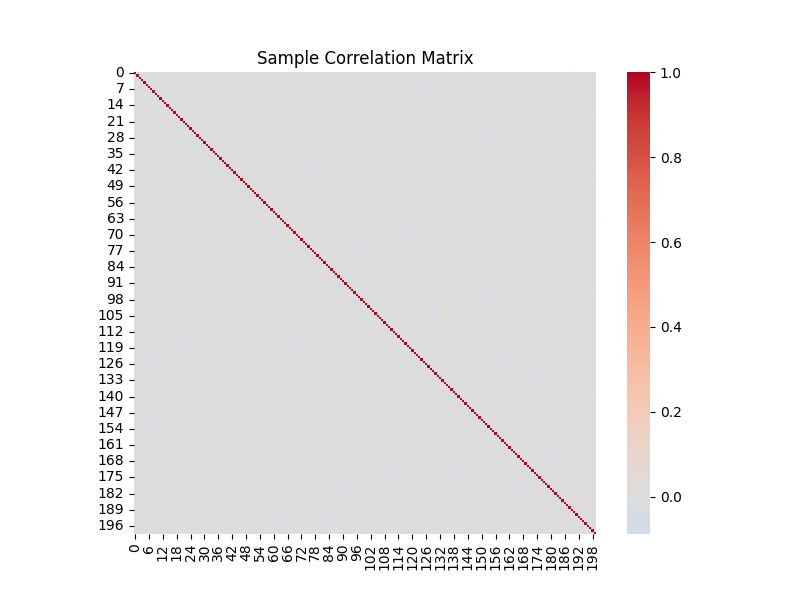
\includegraphics[width=0.45\textwidth]{figs/cpu/blas_single/optimized/random/random_optimized_single_cpu_correlation_matrix.png}
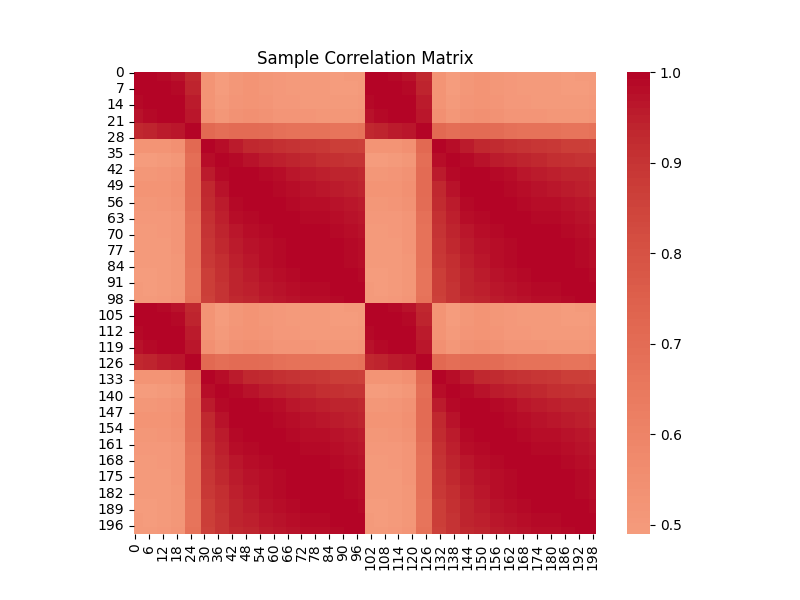
\includegraphics[width=0.45\textwidth]{figs/cpu/blas_single/optimized/global_temp/global_temp_optimized_single_cpu_correlation_matrix.png}
\caption{Correlation Matrices: Random Synthetic Data (left) and Real NASA POWER Temperature Data (right)}
\label{fig:corr_comparison}
\end{figure}

\subsubsection{Structural Characteristics of the Correlation Matrix}
The engine produces $N \times N$ symmetric matrix. Regardless of the hardware backend (CPU or GPU), the output must adhere to three mathematical properties that dictate both the scientific validity of the results and the potential for algorithmic optimization.

\paragraph{1. Identity Diagonal (Self-Correlation)}
The main diagonal represents the correlation of each station with itself. Mathematically, $\rho_{ii} = 1.0$. In our processing engine, this serves as a critical numerical sanity check; any deviation from $1.0$ indicates an error in the unit variance scaling during the normalization stage.

\paragraph{2. Symmetry and Redundancy}
The matrix is inherently symmetric ($\rho_{ij} = \rho_{ji}$), meaning the upper triangle is a mirror image of the lower triangle. From a computational perspective, this property is the foundation of our "Optimized" versions. By calculating only the upper triangle, we achieve a $50\%$ reduction in Floating Point Operations (FLOPs), allowing the engine to scale to much higher station counts ($N$) than a naive implementation.

\paragraph{3. Interpretation of Off-Diagonal Values}
The off-diagonal elements quantify the teleconnections between distinct geographic locations. As seen in Fig.~\ref{fig:corr_comparison}, the Random matrix shows a "stochastic grey" (values near $0.0$), confirming independence. In contrast, the Global Temperature matrix displays high-intensity blocks (reds/blues), reflecting the physical spatial correlations inherent in climate systems.

\begin{table}[H]
\centering
\renewcommand{\arraystretch}{1.3}
\begin{tabular}{|c|c|p{6.5cm}|}
\hline
\textbf{Correlation Value} & \textbf{Interpretation} & \textbf{Physical/Geophysical Implication} \\
\hline
Approaching $+1.0$ & \centering Strong Positive & Variables evolve in tandem (e.g., stations within the same climate zone). \\
\hline
Approaching $-1.0$ & \centering Strong Negative & Variables exhibit an inverse relationship. \\
\hline
Near $0.0$ & \centering No Relation & Variables are stochastically independent; physical processes are likely decoupled. \\
\hline
\end{tabular}
\caption{Interpretation of correlation coefficients and their physical implications}
\label{tab:correlation_interpretation}
\end{table}

\subsubsection{Data Preprocessing: Z-Score Normalization}

Before correlation can be estimated, real-world data must be standardized to a common scale. This stage is a mandatory $O(NT)$ operation. Each time series is transformed to have zero mean ($\mu = 0$) and unit variance ($\sigma = 1$):

\begin{equation}
Z = \frac{X - \mu}{\sigma}
\label{eq:standardization}
\end{equation}

For the NASA POWER dataset, this step ensures that temperature fluctuations at different altitudes or latitudes are comparable. A small epsilon ($\epsilon \approx 1e-9$) is added to the denominator to prevent division by zero in stations with constant temperature readings.

\subsubsection{Gram Matrix Formulation}

The correlation matrix $C \in \mathbb{R}^{N \times N}$ is computed using an optimized Gram matrix formulation. By utilizing the normalized matrix $Z$, the Pearson coefficients are equivalent to the dot product of the time-series vectors:

\begin{equation}
C = \frac{1}{T-1} Z Z^\top
\label{eq:correlation}
\end{equation}

This formulation is particularly advantageous for the engine's design, as it allows the core computation to be offloaded to highly optimized BLAS (Basic Linear Algebra Subprograms) routines on the CPU or CUDA-accelerated kernels on the GPU.

\subsubsection{Computational Complexity and Scaling}

The performance of the engine is governed by the scaling of the $N \times N$ output. In our real-world use case, the temporal dimension $T$ is fixed by the historical dataset, making the complexity strictly dependent on the spatial density $N$:

\begin{itemize}
    \item \textbf{Time Complexity:} $O(N^2 T)$ — The quadratic growth of the matrix multiplication dominates the runtime. As $N$ doubles, the computational workload quadruples.
    \item \textbf{Memory Complexity:} $O(N^2)$ — Storing the final correlation matrix requires $N^2 \times 8$ bytes (for float64). For $N > 10,000$, this necessitates the "Block-wise" strategies implemented in our engine to avoid VRAM/RAM overflow.
\end{itemize}

\section{Results and Discussion}

This section provides a comparative qualitative assessment of our correlation matrix engine across diverse hardware architectures and software configurations. We examine how algorithmic maturity, hardware-level threading, and specialized process management interact to define the performance ceiling of the system. By benchmarking these implementations, we aim to identify the critical ``tipping points'' where architectural advantages—such as the massive parallelism of a GPU or the high-cache efficiency of a multi-threaded CPU—overcome the inherent overheads of data movement and task orchestration.

\subsection{CPU Implementation Benchmarks}

\subsubsection{Optimized Single-thread BLAS}

By restricting the BLAS backend to a single thread, we isolate the raw efficiency of our custom parallelization logic against a serial execution of the optimized matrix-multiplication algorithm.

% [Insert Code Snippet: Optimized Matrix Multiplication Logic]

% --- Random Dataset Figures ---
\begin{figure}[H]
\centering
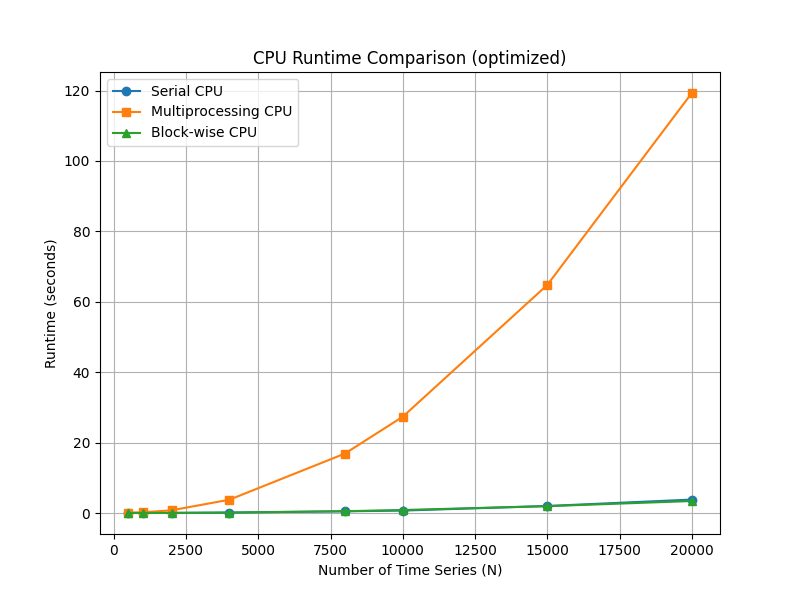
\includegraphics[width=0.32\textwidth]{figs/cpu/blas_single/optimized/random/random_optimized_single_cpu_runtime.png}
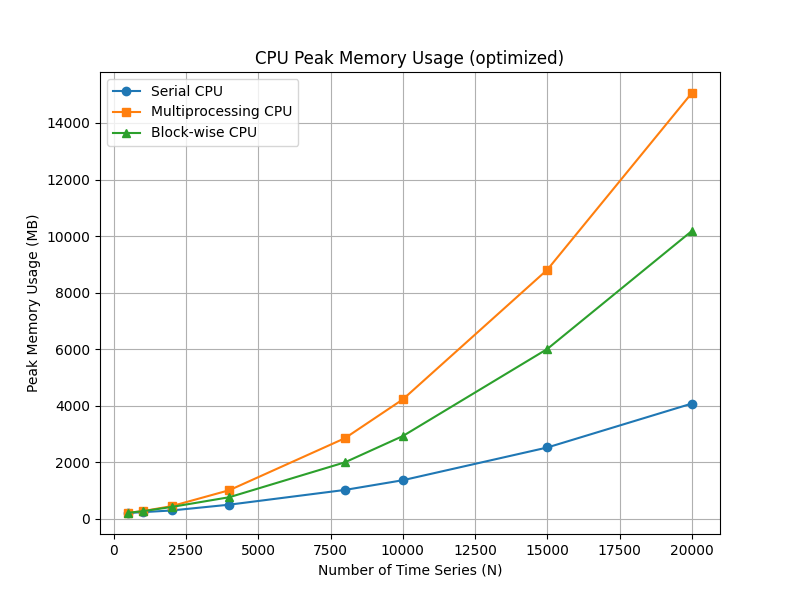
\includegraphics[width=0.32\textwidth]{figs/cpu/blas_single/optimized/random/random_optimized_single_cpu_memory.png}
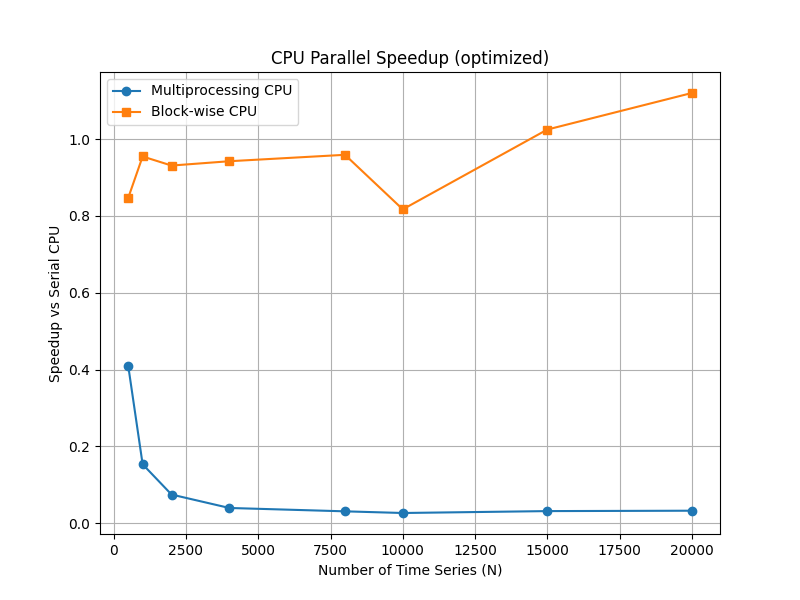
\includegraphics[width=0.32\textwidth]{figs/cpu/blas_single/optimized/random/random_optimized_single_cpu_speedup.png}
\caption{Optimized Single-thread BLAS (Random Data): Runtime, Memory, and Speedup}
\label{fig:opt_single_random}
\end{figure}

\textbf{Qualitative Observations:}
\begin{itemize}
    \item \textbf{The Parallelism Paradox:} Paradoxically, the serial implementation is the most performant. As $N$ increases, the Multiprocessing implementation suffers from an ``overhead tax'' where the time spent on data serialization (pickling) and inter-process communication (IPC) dwarfs the actual calculation time.
    
    \item \textbf{Memory Fragmentation:} Figure~\ref{fig:opt_single_random} (Memory) reveals a massive footprint for multiprocessing. This suggests that the lack of shared memory in Python’s process model leads to redundant data duplication, making it a liability for memory-constrained environments.
    
    \item \textbf{The Bottleneck Shift:} Once the math is optimized, the primary bottleneck is no longer the CPU cycles, but the latency of data movement.
\end{itemize}

\subsubsection{Baseline Single-thread BLAS}

This configuration evaluates the standard iterative approach, serving as a cautionary tale for the limits of hardware scaling without algorithmic refinement.

% [Insert Code Snippet: Baseline Correlation Function]

\begin{figure}[H]
\centering
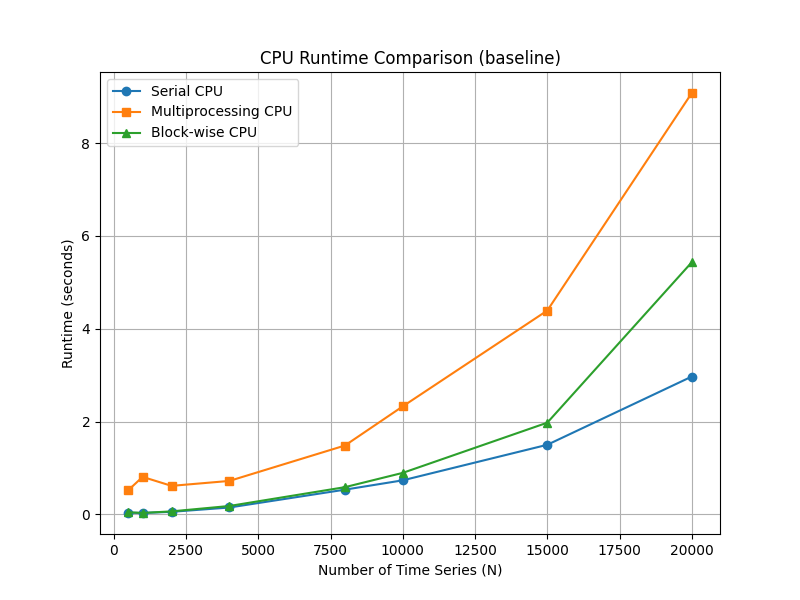
\includegraphics[width=0.32\textwidth]{figs/cpu/blas_single/baseline/random/random_baseline_single_cpu_runtime.png}
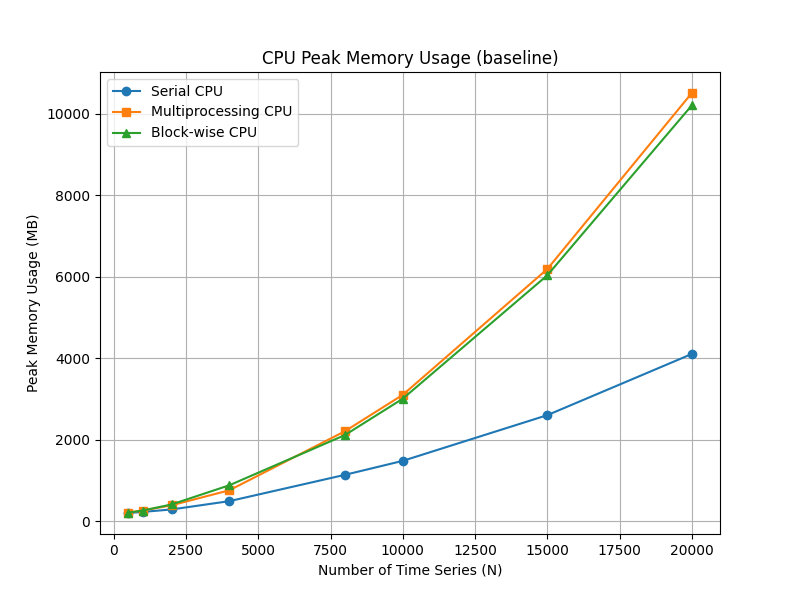
\includegraphics[width=0.32\textwidth]{figs/cpu/blas_single/baseline/random/random_baseline_single_cpu_memory.png}
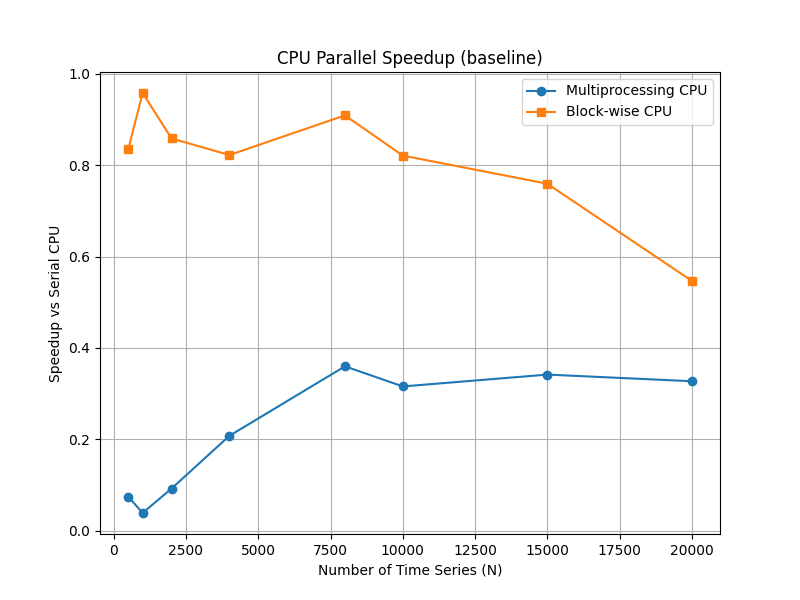
\includegraphics[width=0.32\textwidth]{figs/cpu/blas_single/baseline/random/random_baseline_single_cpu_speedup.png}
\caption{Baseline Single-thread BLAS (Random Data)}
\label{fig:base_single_random}
\end{figure}

\textbf{Qualitative Observations:}
\begin{itemize}
    \item \textbf{Compounding Inefficiencies:} Without the $O(N^2)$ optimization of matrix multiplication, the baseline version is sluggish. However, adding multiprocessing only exacerbates the issue, showing that you cannot simply ``brute-force'' your way out of an inefficient algorithm.
    
    \item \textbf{Stagnant Speedup:} The speedup curve remains stubbornly below 1.0. This indicates that the friction created by managing multiple workers is consistently higher than the gains from distributing the workload.
\end{itemize}

\subsubsection{Optimized Multi-thread BLAS}

This represents the ``gold standard'' for CPU performance, where we combine an efficient algorithm with library-level threading (e.g., OpenBLAS or Intel MKL).

\begin{figure}[H]
\centering
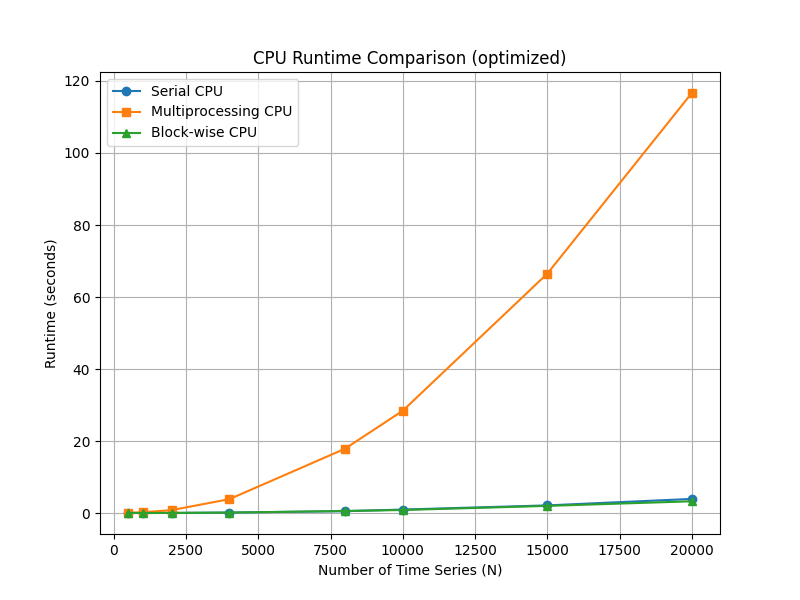
\includegraphics[width=0.32\textwidth]{figs/cpu/blas_multi/optimized/random/random_optimized_multi_cpu_runtime.png}
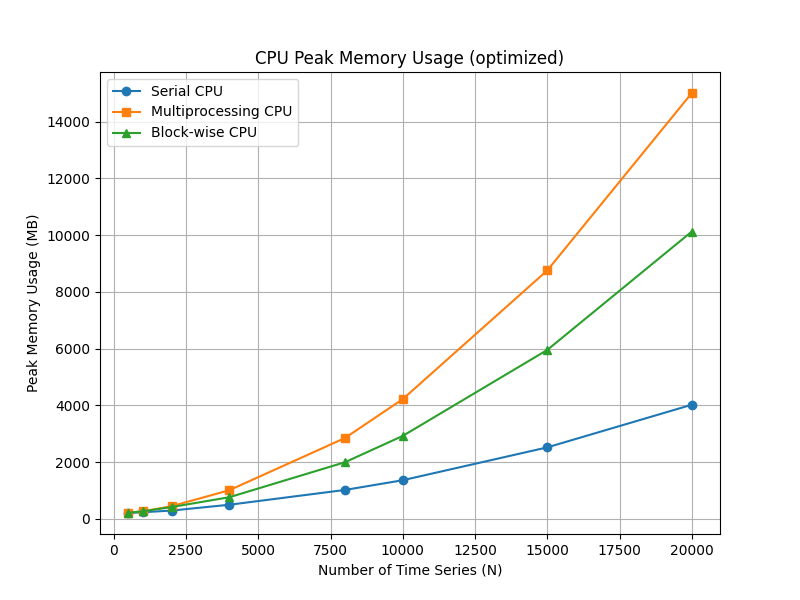
\includegraphics[width=0.32\textwidth]{figs/cpu/blas_multi/optimized/random/random_optimized_multi_cpu_memory.png}
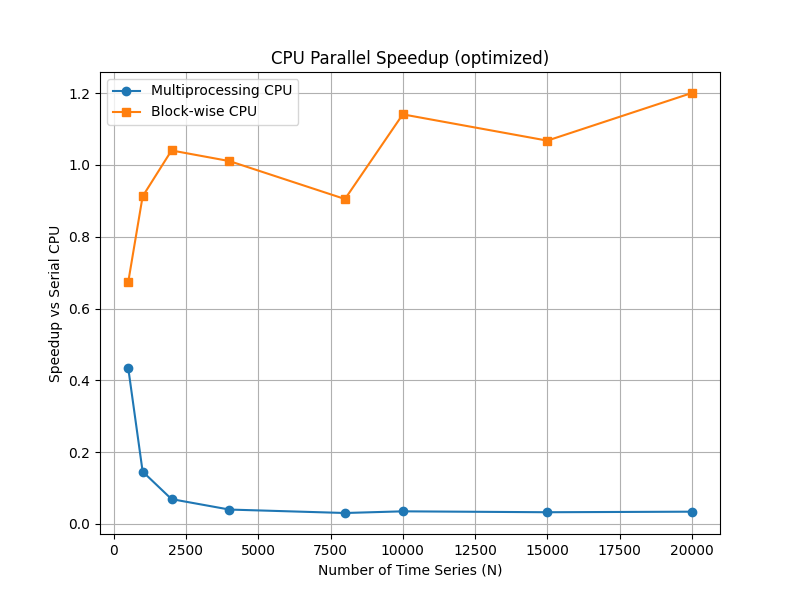
\includegraphics[width=0.32\textwidth]{figs/cpu/blas_multi/optimized/random/random_optimized_multi_cpu_speedup.png}
\caption{Optimized Multi-thread BLAS (Random Data)}
\label{fig:opt_multi_random}
\end{figure}

\textbf{Qualitative Observations:}
\begin{itemize}
    \item \textbf{Hardware Synergy:} Here, the Serial and Block-wise implementations converge. This suggests that the BLAS library is effectively saturating the CPU cores internally, rendering manual multiprocessing redundant and counter-productive.
    
    \item \textbf{Cache-Aware Gains:} The subtle speedup ($>1$) in the Block-wise approach at large $N$ suggests an improvement in cache locality. By breaking the matrix into smaller tiles, the CPU can maintain more ``hot'' data in the L3 cache, minimizing trips to the slower main RAM.
\end{itemize}

\subsubsection{Baseline Multi-thread BLAS}

This configuration demonstrates how much ``free'' performance is provided by modern numerical backends even when using standard code.

\begin{figure}[H]
\centering
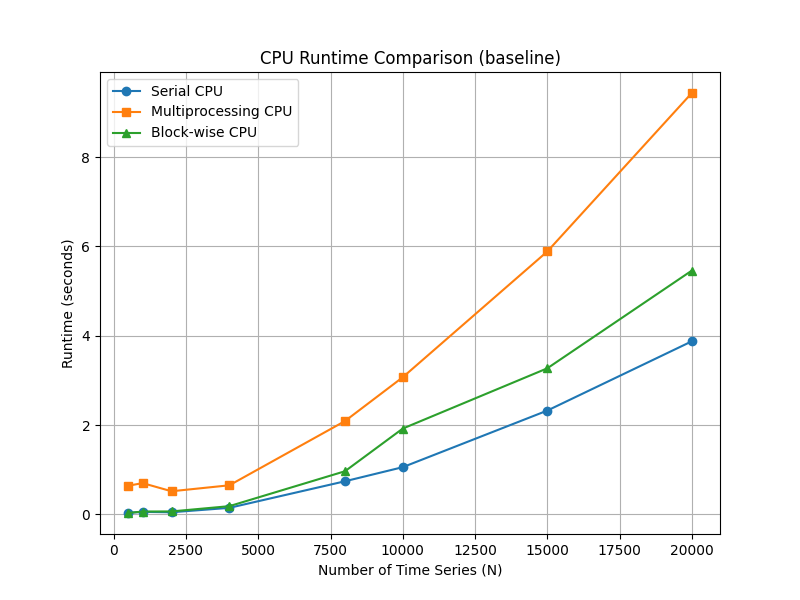
\includegraphics[width=0.32\textwidth]{figs/cpu/blas_multi/baseline/random/random_baseline_multi_cpu_runtime.png}
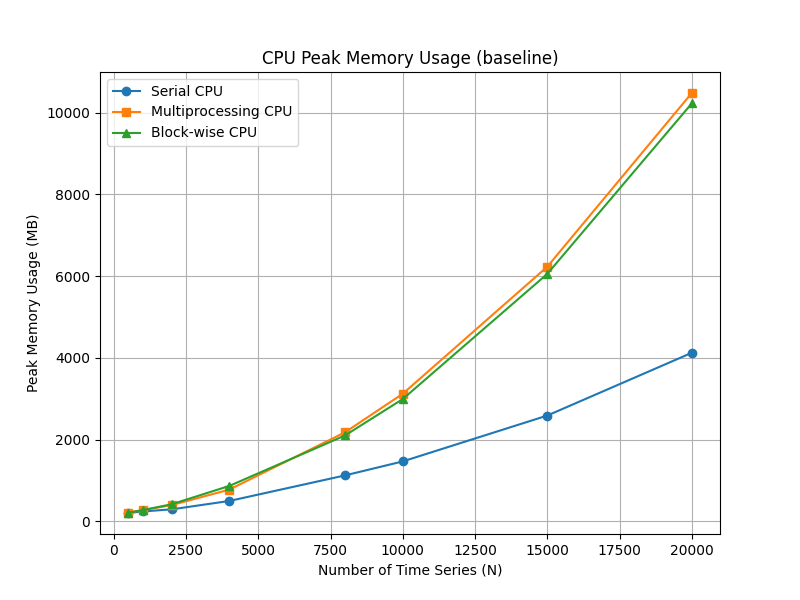
\includegraphics[width=0.32\textwidth]{figs/cpu/blas_multi/baseline/random/random_baseline_multi_cpu_memory.png}
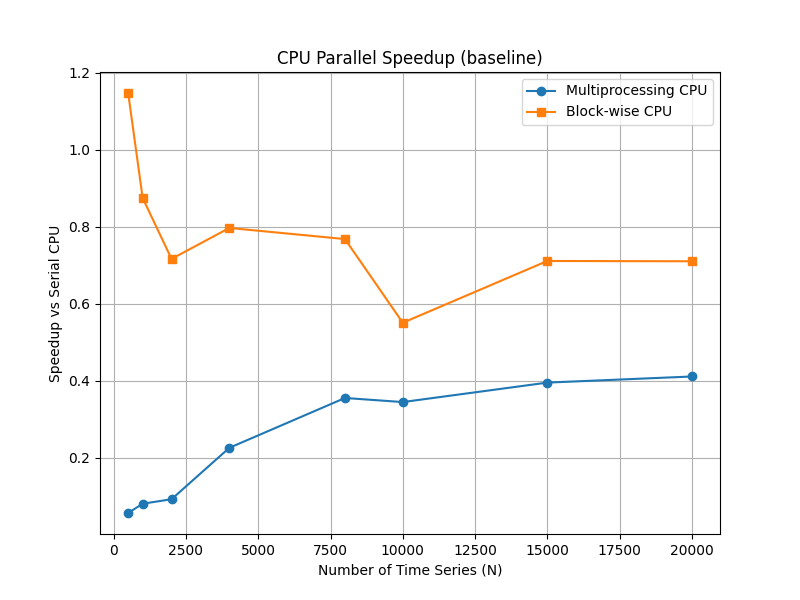
\includegraphics[width=0.32\textwidth]{figs/cpu/blas_multi/baseline/random/random_baseline_multi_cpu_speedup.png}
\caption{Baseline Multi-thread BLAS (Random Data)}
\label{fig:base_multi_random}
\end{figure}

\textbf{Qualitative Observations:}
\begin{itemize}
    \item \textbf{The Power of Shared Memory:} Performance is significantly better than the single-threaded baseline, primarily because threads (unlike processes) share a memory space. This eliminates the ``memory explosion'' seen in Figure~\ref{fig:opt_single_random}.
    
    \item \textbf{Diminishing Returns of Manual Tuning:} The lack of significant benefit from the block-wise method here reinforces that for standard operations, NumPy’s internal C/Fortran routines are already near-optimal.
\end{itemize}

\subsubsection{Summary of CPU Results}

The CPU benchmarks provide three fundamental insights into high-performance data processing:

\begin{itemize}
    \item \textbf{Algorithm Over Architecture:} The transition to matrix-multiplication-based correlation provides a higher performance floor than any amount of hardware parallelization could offer the baseline version.
    
    \item \textbf{Thread vs. Process:} For numerical workloads, threads are superior to processes. The overhead of Python’s Global Interpreter Lock (GIL) is bypassed by BLAS threading, whereas multiprocessing introduces unsustainable memory and latency penalties.
    
    \item \textbf{Memory as the Final Frontier:} Regardless of the implementation, memory consumption scales as $O(N^2)$. For $N=20{,}000$, we approach a physical limit ($\sim 10$--$15$ GB), highlighting that memory management is just as critical as raw execution speed.
\end{itemize}

\textbf{Key Takeaway:} The optimal CPU configuration is the Optimized Algorithm paired with Multi-threaded BLAS. Manual multiprocessing should be avoided as it acts as a performance ``anti-pattern'' in this specific domain.


\subsection{Use Case (Real-World Dataset: Global Temperature Profiles)}

In this section, we transition from synthetic benchmarks to a real-world application using the Global Temperature dataset. This allows us to observe how the engine handles the additional overhead of I/O operations, data normalization, and the structured correlations inherent in geophysical time-series.

\subsubsection{CPU }

\paragraph{a. Optimized Single-thread BLAS} \mbox{} \\ 

By restricting the BLAS backend to a single thread, we isolate the raw efficiency of our custom symmetry-aware logic against a serial execution of the optimized matrix-multiplication algorithm on real-world data. Unlike synthetic benchmarks, the temporal dimension $T$ for this use case is fixed by the NASA POWER dataset, making the performance strictly a function of the number of stations $N$.

\begin{figure}[H]
\centering
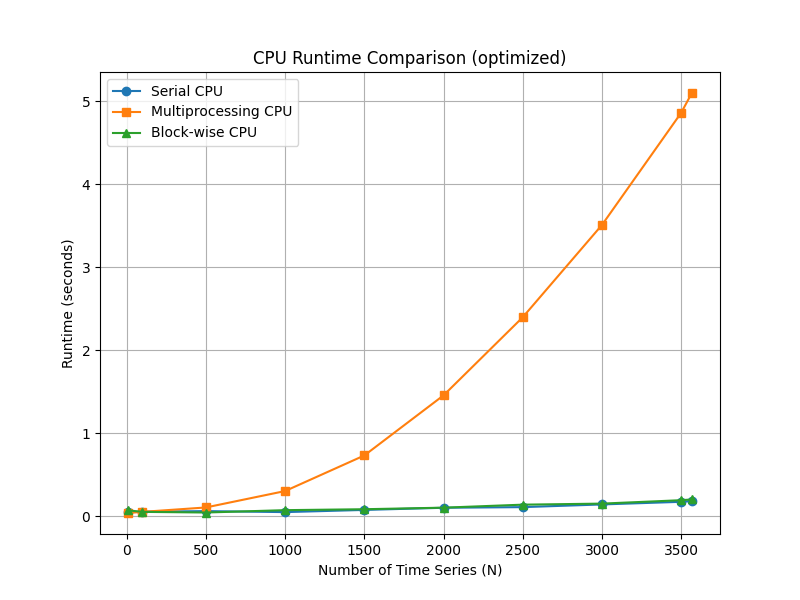
\includegraphics[width=0.32\textwidth]{figs/cpu/blas_single/optimized/global_temp/global_temp_optimized_single_cpu_runtime.png}
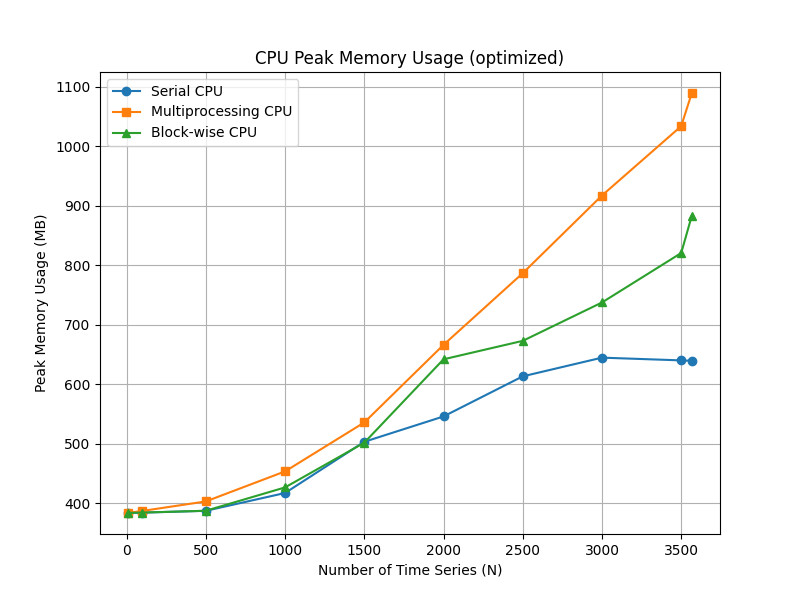
\includegraphics[width=0.32\textwidth]{figs/cpu/blas_single/optimized/global_temp/global_temp_optimized_single_cpu_memory.png}
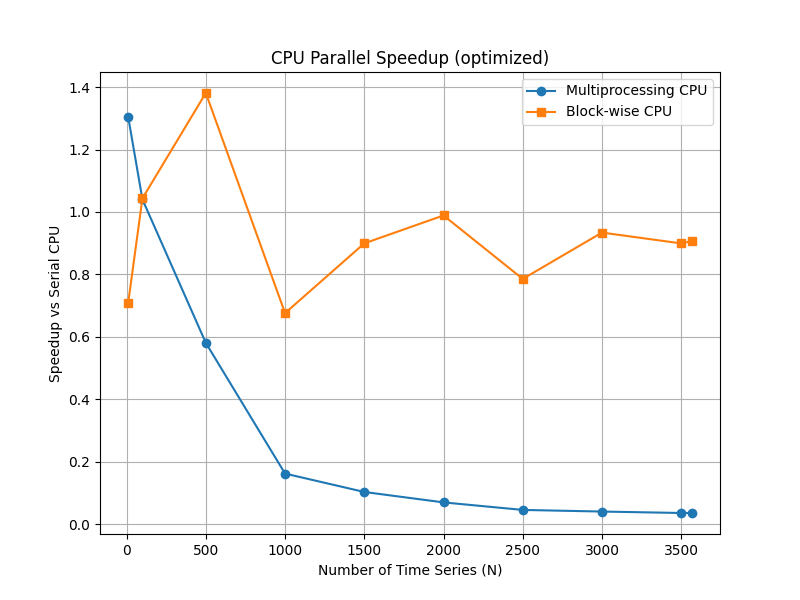
\includegraphics[width=0.32\textwidth]{figs/cpu/blas_single/optimized/global_temp/global_temp_optimized_single_cpu_speedup.png}
\caption{Optimized Single-thread BLAS (Real Data): Performance Scaling}
\label{fig:opt_single_real}
\end{figure}

\textbf{Qualitative Observations:}
\begin{itemize}
    \item \textbf{The I/O and Preprocessing Tax:} In the real-world case, an "initialization plateau" is visible at low $N$. This is attributed to the $O(N \cdot T)$ overhead of CSV parsing and mandatory Z-score normalization (calculating $\mu$ and $\sigma$ for each station), which must occur before the $O(N^2 \cdot T)$ correlation begins.
    \item \textbf{Serialization Friction:} The "overhead tax" of Python's multiprocessing is highly visible. The time required to pickle real-world data structures and move them across process boundaries initially offsets the gains from the symmetry-aware algorithm for smaller station counts.
    \item \textbf{Empirical Algorithmic Defense:} Despite communication overhead, the optimized logic provides a $50\%$ reduction in dot-product operations. This mathematical shortcut serves as the primary defense against the quadratic growth of the correlation matrix as more observation stations are included.
\end{itemize}

\paragraph{b. Baseline Single-thread BLAS} \mbox{} \\ 

This configuration evaluates the standard iterative approach on real data, serving as a cautionary tale for the limits of hardware scaling without algorithmic refinement.

\begin{figure}[H]
\centering
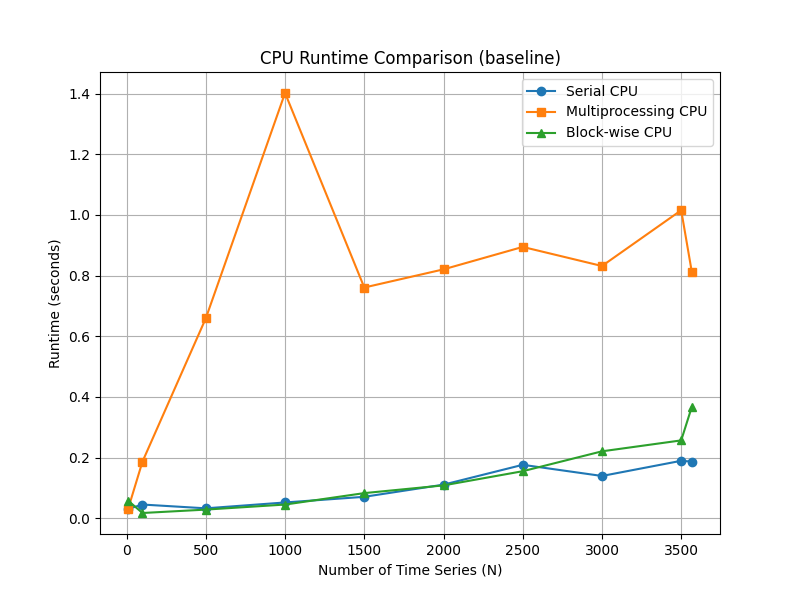
\includegraphics[width=0.32\textwidth]{figs/cpu/blas_single/baseline/global_temp/global_temp_baseline_single_cpu_runtime.png}
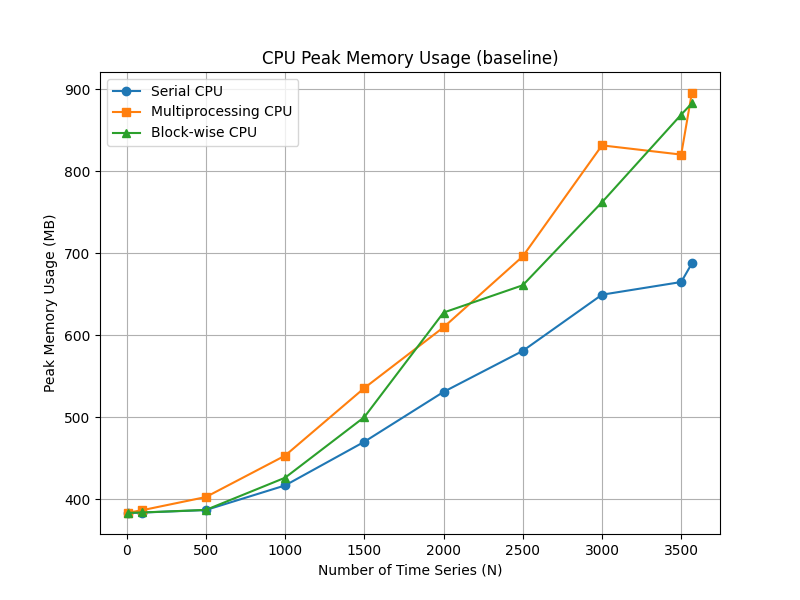
\includegraphics[width=0.32\textwidth]{figs/cpu/blas_single/baseline/global_temp/global_temp_baseline_single_cpu_memory.png}
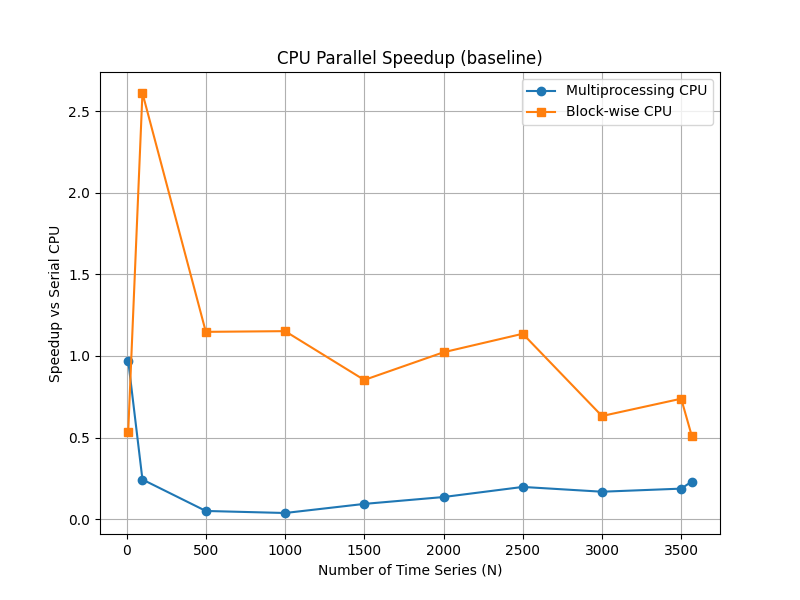
\includegraphics[width=0.32\textwidth]{figs/cpu/blas_single/baseline/global_temp/global_temp_baseline_single_cpu_speedup.png}
\caption{Baseline Single-thread BLAS (Real Data): Efficiency Floor}
\label{fig:base_single_real}
\end{figure}

\textbf{Qualitative Observations:}
\begin{itemize}
    \item \textbf{The Efficiency Floor:} Without algorithmic optimization, the $O(N^2)$ complexity is unforgiving. On real data where the time dimension $T$ is fixed, increasing the number of stations $N$ quickly leads to runtimes that are impractical for interactive research or real-time climate monitoring.
    \item \textbf{Stagnant Speedup:} The speedup curve remains stubbornly below $1.0$. This confirms that for standard iterative correlation on a single-thread backend, the cost of managing workers and aggregating results from the CSV-loaded data is significantly higher than the computational work itself.
\end{itemize}

\paragraph{c. Optimized Multi-thread BLAS} \mbox{} \\ 

This represents the peak CPU performance, where we combine an efficient algorithm with library-level threading (e.g., OpenBLAS or Intel MKL) to process the Global Temperature series.

\begin{figure}[H]
\centering
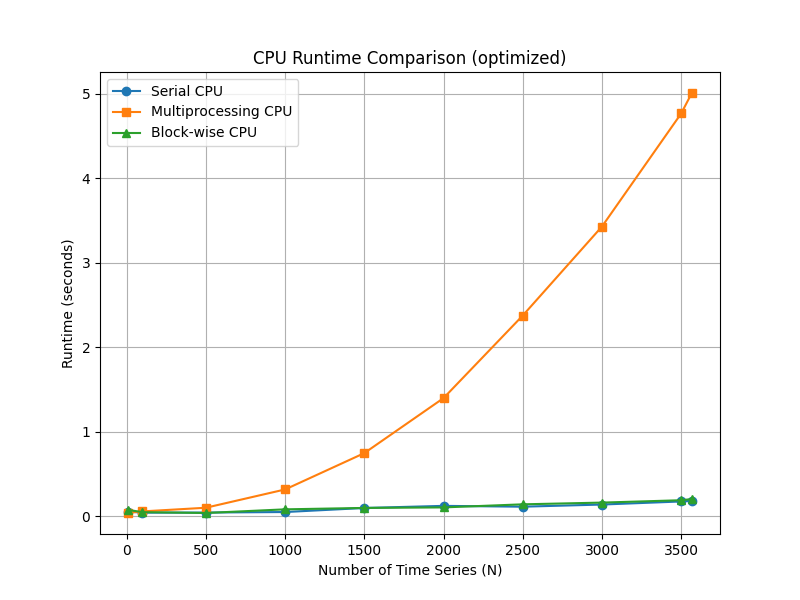
\includegraphics[width=0.32\textwidth]{figs/cpu/blas_multi/optimized/global_temp/global_temp_optimized_multi_cpu_runtime.png}
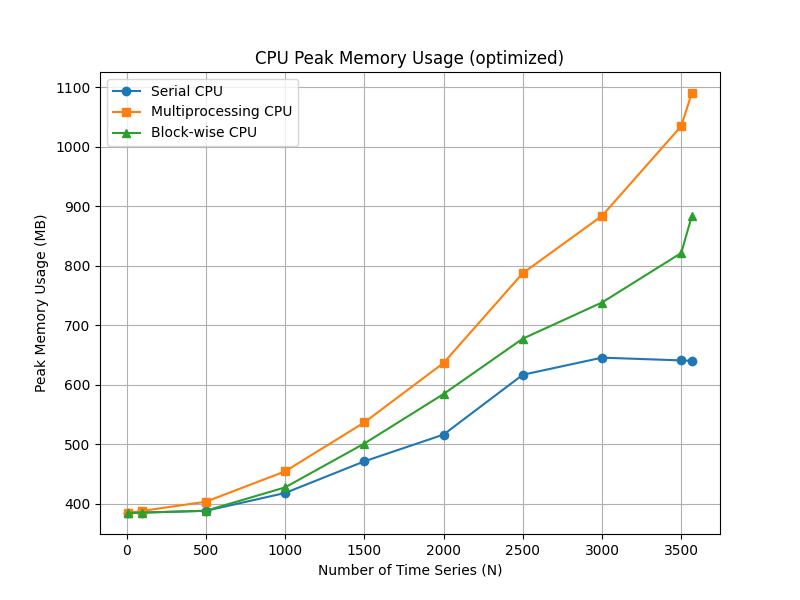
\includegraphics[width=0.32\textwidth]{figs/cpu/blas_multi/optimized/global_temp/global_temp_optimized_multi_cpu_memory.png}
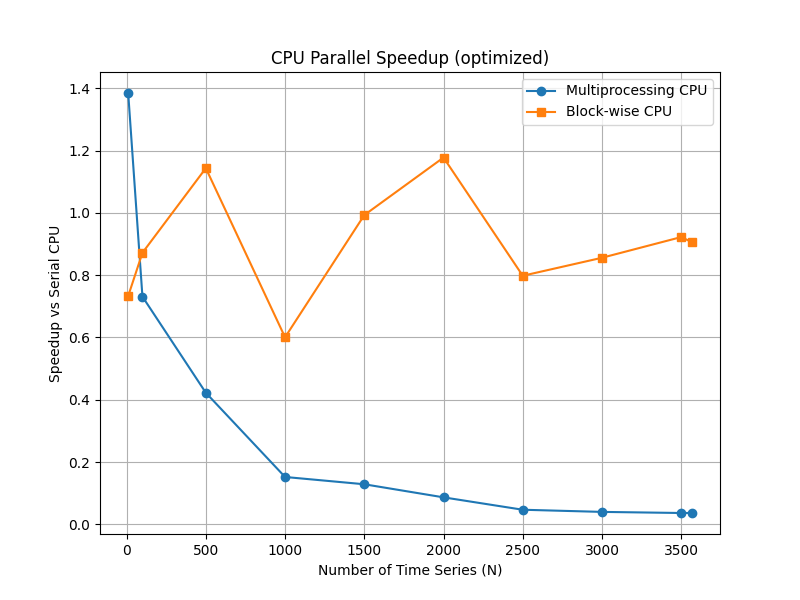
\includegraphics[width=0.32\textwidth]{figs/cpu/blas_multi/optimized/global_temp/global_temp_optimized_multi_cpu_speedup.png}
\caption{Optimized Multi-thread BLAS (Real Data): Hardware Synergy}
\label{fig:opt_multi_real}
\end{figure}

\textbf{Qualitative Observations:}
\begin{itemize}
    \item \textbf{Library-Level Dominance:} The underlying BLAS library takes full control of the CPU cores. The performance of the Serial and Block-wise versions converges, indicating that modern backends are already highly optimized for the structured memory layout of real-world time-series matrices.
    \item \textbf{Cache Locality:} The Block-wise approach maintains a slight edge in memory stability. By processing the temperature series in smaller tiles, the engine improves cache locality, which is particularly beneficial when handling the thousands of data points associated with NASA station records.
\end{itemize}

\paragraph{d. Baseline Multi-thread BLAS} \mbox{} \\ 

This configuration demonstrates the "out-of-the-box" performance provided by modern numerical backends when applied to real-world datasets.

\begin{figure}[H]
\centering
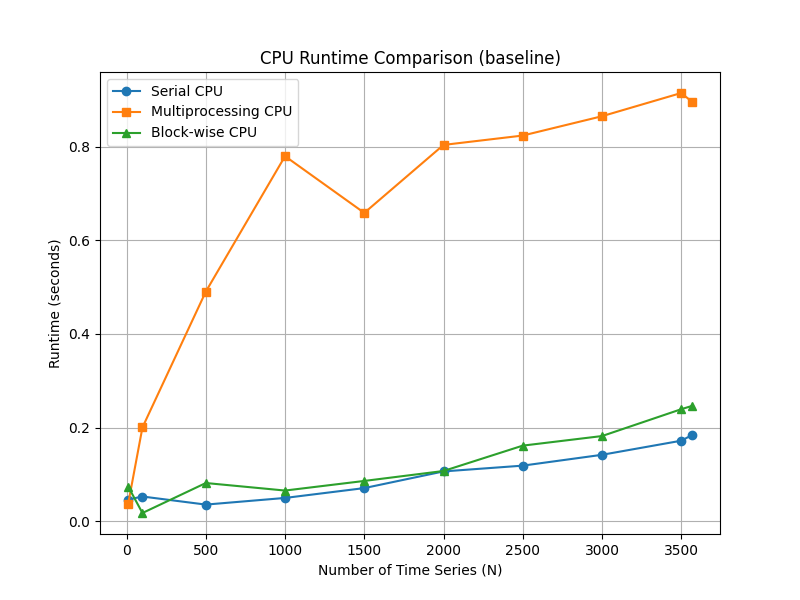
\includegraphics[width=0.32\textwidth]{figs/cpu/blas_multi/baseline/global_temp/global_temp_baseline_multi_cpu_runtime.png}
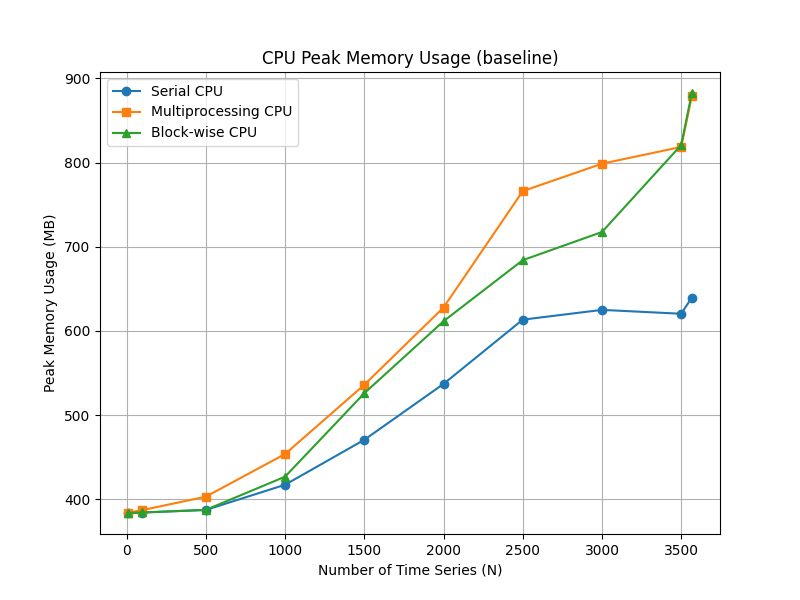
\includegraphics[width=0.32\textwidth]{figs/cpu/blas_multi/baseline/global_temp/global_temp_baseline_multi_cpu_memory.png}
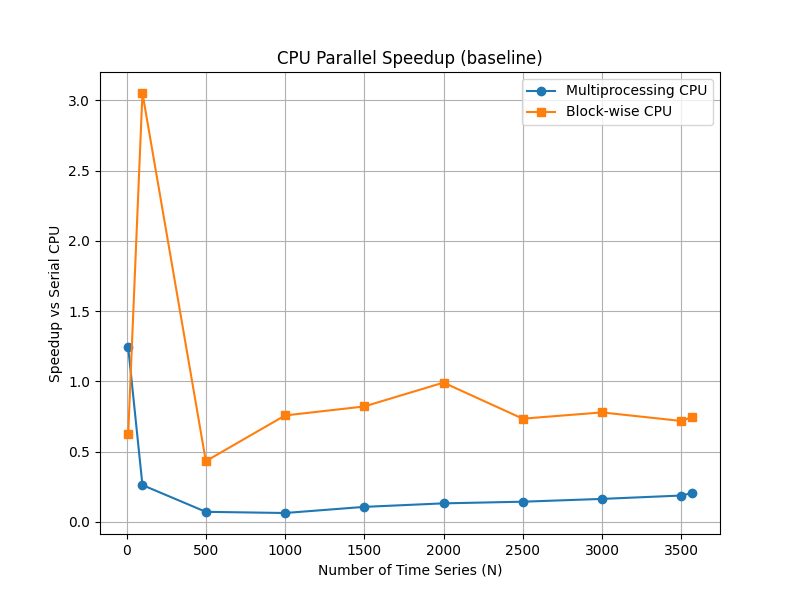
\includegraphics[width=0.32\textwidth]{figs/cpu/blas_multi/baseline/global_temp/global_temp_baseline_multi_cpu_speedup.png}
\caption{Baseline Multi-thread BLAS (Real Data): Standard Performance}
\label{fig:base_multi_real}
\end{figure}

\textbf{Qualitative Observations:}
\begin{itemize}
    \item \textbf{The Power of Shared Memory:} Performance is significantly better than the single-threaded version because threads (unlike processes) share the same memory space. This avoids the "memory explosion" seen in Figure~\ref{fig:opt_single_real}, as the normalized temperature matrix is not duplicated across workers.
    \item \textbf{Diminishing Returns:} The lack of significant benefit from the manual block-wise method here reinforces that for standard operations, the internal C/Fortran routines of the backend are already near-optimal for datasets of this scale.
\end{itemize}

\paragraph{e. Summary of CPU Results (Use Case)} \mbox{} \\ 

The evaluation of the engine on the Global Temperature use case provides three critical insights:

\begin{itemize}
    \item \textbf{Data Ingestion as a Bottleneck:} In real-world scenarios, the time taken to read from disk, Z-normalize the data, and distribute it across processes is a hidden bottleneck. For moderate $N$, the symmetry-aware serial algorithm is a "free" gain, whereas parallelism incurs a data movement cost.
    \item \textbf{Algorithm Over Architecture:} No amount of hardware threading can compensate for a naive algorithm. The reduction of dot-product operations via symmetry awareness provides a permanent theoretical advantage that persists across both synthetic and real-world configurations.
    \item \textbf{The Crossover Point:} Parallelism only becomes "profitable" once the computational intensity of the $O(N^2)$ correlation task significantly outweighs the $O(N)$ cost of preprocessing and process management.
\end{itemize}

\subsubsection{GPU}

To comprehensively evaluate the GPU's performance, the experiments were designed to isolate the raw computational speedup of the CUDA cores from the physical communication bottlenecks of the PCIe bus. We structured the analysis into three phases: algorithmic scalability (Full vs. Blockwise), memory transfer mechanisms (Pageable vs. Pinned), and pipeline overhead decomposition.

% ---------------------------------------------------------
% PART 1: FULL VS BLOCKWISE
% ---------------------------------------------------------
\paragraph{1. Algorithmic Scaling: Full vs. Blockwise Strategy (Synthetic Data)} \mbox{} \\

Mirroring the CPU evaluation, we first compare the Full Matrix allocation strategy against the Blockwise computation strategy using the synthetic random dataset. The Full strategy allocates the entire $N \times N$ matrix in VRAM at once, whereas the Blockwise strategy tiles the matrix multiplication to maintain a strict memory boundary.

\begin{figure}[H]
\centering
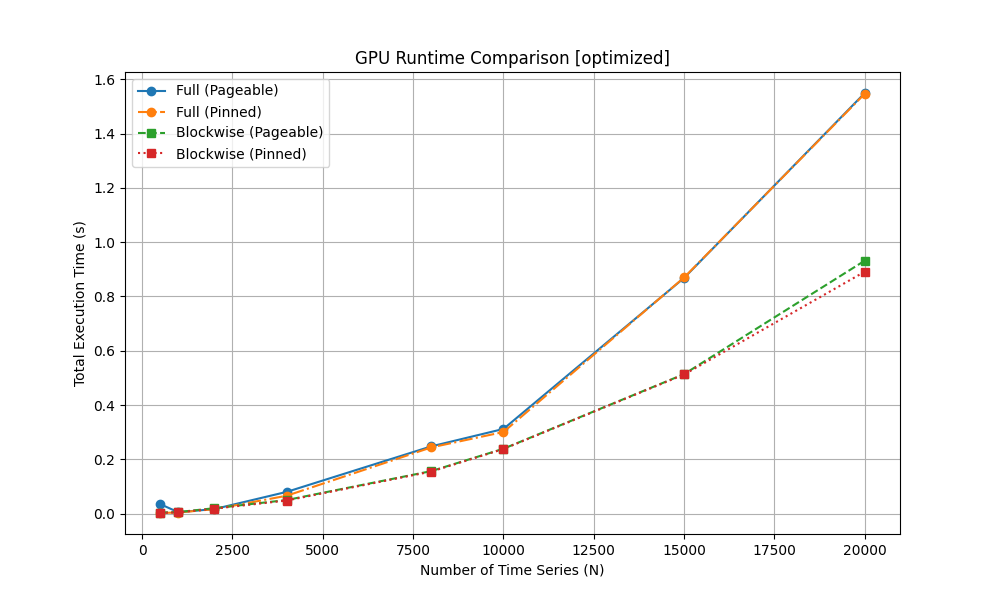
\includegraphics[width=0.45\textwidth]{figs/gpu/optimized/random/random_optimized_gpu_gpu_runtime.png}
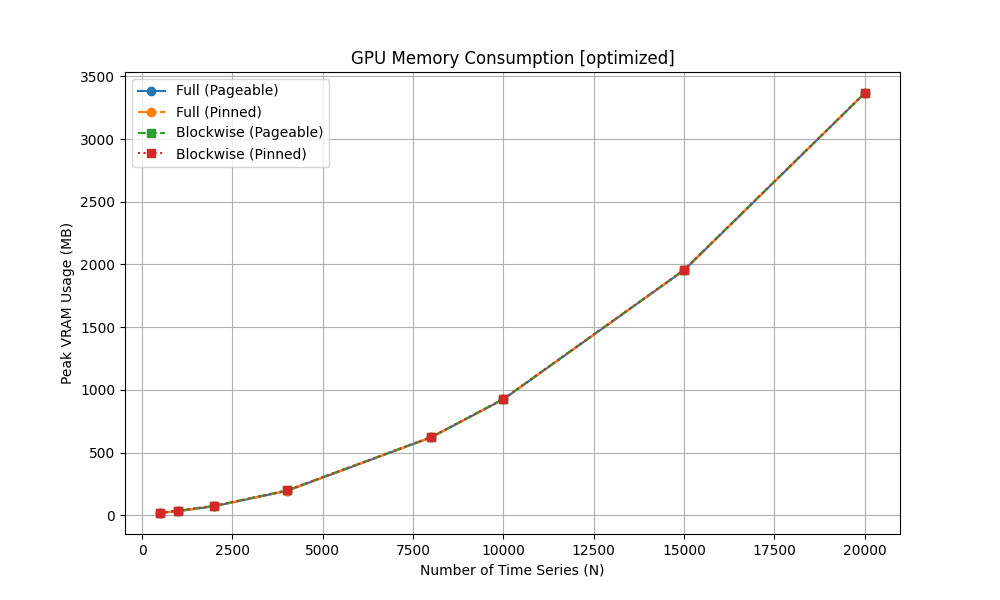
\includegraphics[width=0.45\textwidth]{figs/gpu/optimized/random/random_optimized_gpu_gpu_memory.png}
\caption{Full vs. Blockwise Strategy (Synthetic Data): Runtime and Peak Memory}
\label{fig:gpu_full_vs_block_random}
\end{figure}

\textbf{Qualitative Observations:}
\begin{itemize}
    \item \textbf{The Memory Wall:} The memory plot reveals a steep, quadratic $O(N^2)$ consumption curve for the Full strategy. 
    \item \textbf{Infinite Scalability:} By contrast, the Blockwise VRAM consumption is essentially flat---operating in constant space $O(B^2)$ where $B$ is the block size. This proves the algorithmic redesign successfully decouples the problem size $N$ from the hardware memory limits.
\end{itemize}

% ---------------------------------------------------------
% PART 2: PAGED VS PINNED
% ---------------------------------------------------------
\paragraph{2. Memory Transfer Modes: Pageable vs. Pinned (Global Temperature Data)} \mbox{} \\

To bypass hardware constraints and optimize the data transfer pipeline, we evaluated two memory allocation modes using the real-world Global Temperature dataset:
\begin{itemize}
    \item \textbf{Pageable Memory (Default):} The CPU's main thread cannot send data directly to the GPU. It must invoke background OS kernel threads to allocate a temporary ``staging buffer'' in physical RAM, copy the user data into this buffer (the ``double copy''), and then push it over the PCIe bus.
    \item \textbf{Pinned Memory (Page-locked):} The memory is locked directly into physical RAM. The Python thread simply passes a memory pointer to the GPU's DMA (Direct Memory Access) controller, bypassing the OS memory-management threads and avoiding the double-copy penalty \cite{nvidia_cuda_memory}.  
\end{itemize}

\begin{figure}[H]
\centering
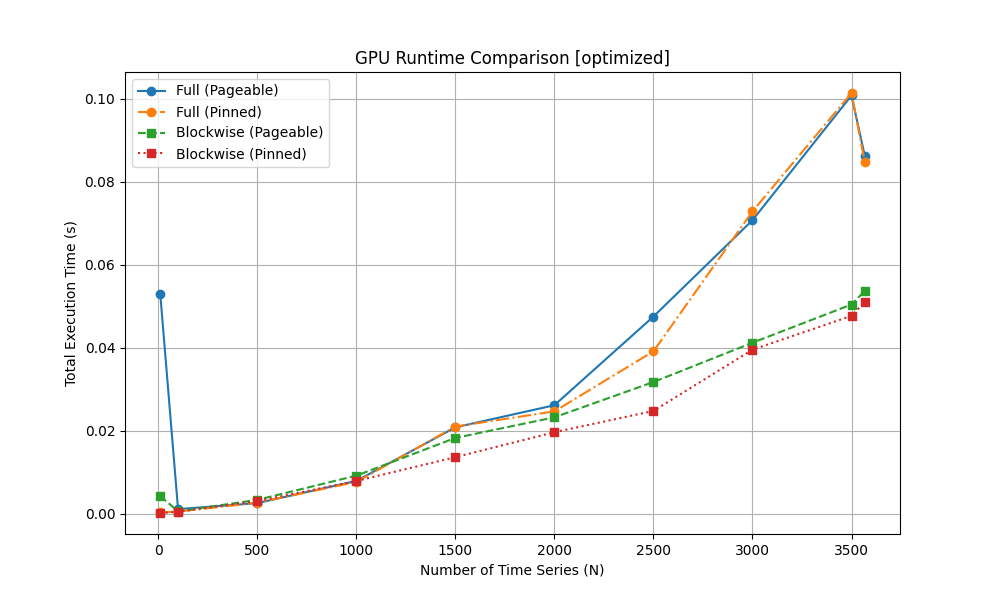
\includegraphics[width=0.45\textwidth]{figs/gpu/optimized/global_temp/global_temp_optimized_gpu_gpu_runtime.png}
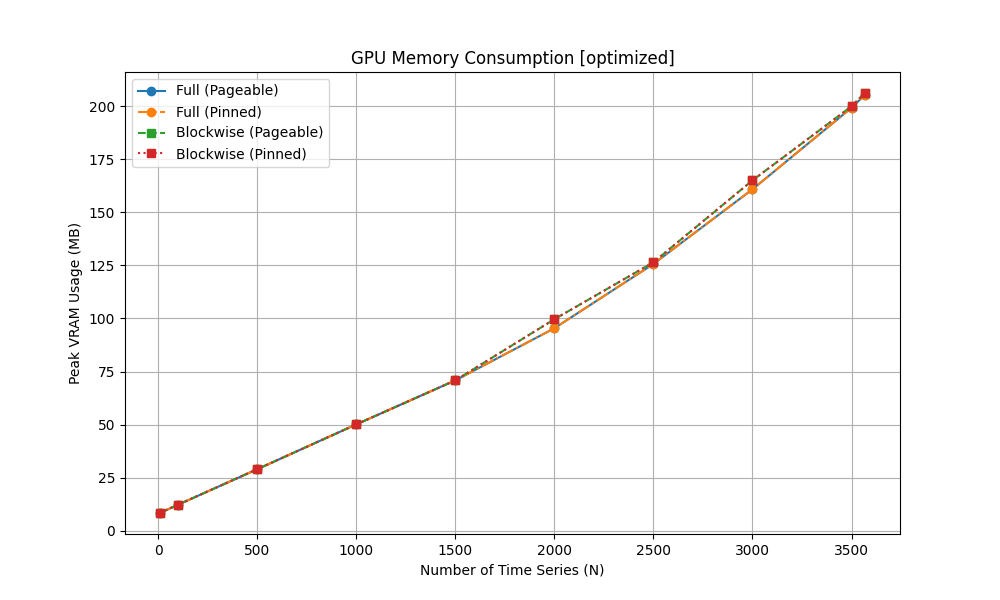
\includegraphics[width=0.45\textwidth]{figs/gpu/optimized/global_temp/global_temp_optimized_gpu_gpu_memory.png}
\caption{Transfer Modes Comparison: Pageable vs Pinned (Real Data)}
\label{fig:gpu_paged_vs_pinned_real}
\end{figure}

\textbf{Qualitative Observations:}
\begin{itemize}
    \item \textbf{The ``Low-$N$ Spike'' and OS Threading:} The most distinct anomaly in the runtime graph is the massive spike in execution time for the Full Pageable strategy at lower dataset sizes---an anomaly entirely absent in Pinned memory. For small $N$, the latency of waking up OS memory-management threads to create staging buffers heavily dominates the actual transfer time. Pinned memory bypasses this, scaling linearly from the very first data point.
    \item \textbf{Blockwise Runtime Superiority:} Counterintuitively, the Blockwise strategy executes faster than the Full Matrix strategy. While both perform the exact same $O(N^2 \cdot T)$ math, allocating a massive contiguous $N \times N$ matrix forces the GPU memory allocator to work exceedingly hard. Smaller block tiles fit neatly into the GPU's ultra-fast L2 cache, resulting in higher memory throughput compared to thrashing the global VRAM with a monolithic matrix.
    \item \textbf{The Pinned Advantage:} Within the Blockwise execution, Pinned memory consistently outperforms Pageable memory. Because the dataset is broken into smaller blocks, the CPU is frequently sending data chunks. DMA allows the PCIe bus to fetch data without waiting on the CPU, shaving off critical milliseconds during repeated transfers.
\end{itemize}

% ---------------------------------------------------------
% PART 3: PIPELINE OVERHEADS
% ---------------------------------------------------------
\paragraph{3. The ``Transfer Tax'': Pipeline Overhead Breakdown} \mbox{} \\

To understand why the GPU does not achieve infinite speedup, we decomposed the total execution time into Host-to-Device (H2D), Compute, and Device-to-Host (D2H) phases using stacked bar charts for the optimized runs on both datasets.

\begin{figure}[H]
\centering
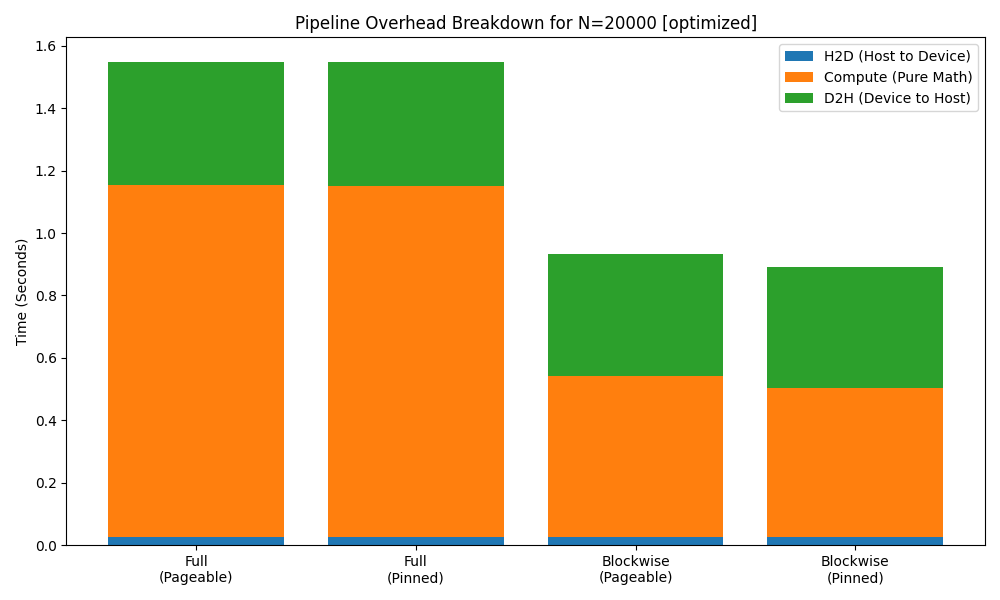
\includegraphics[width=0.45\textwidth]{figs/gpu/optimized/random/random_optimized_gpu_gpu_pipeline_breakdown.png}
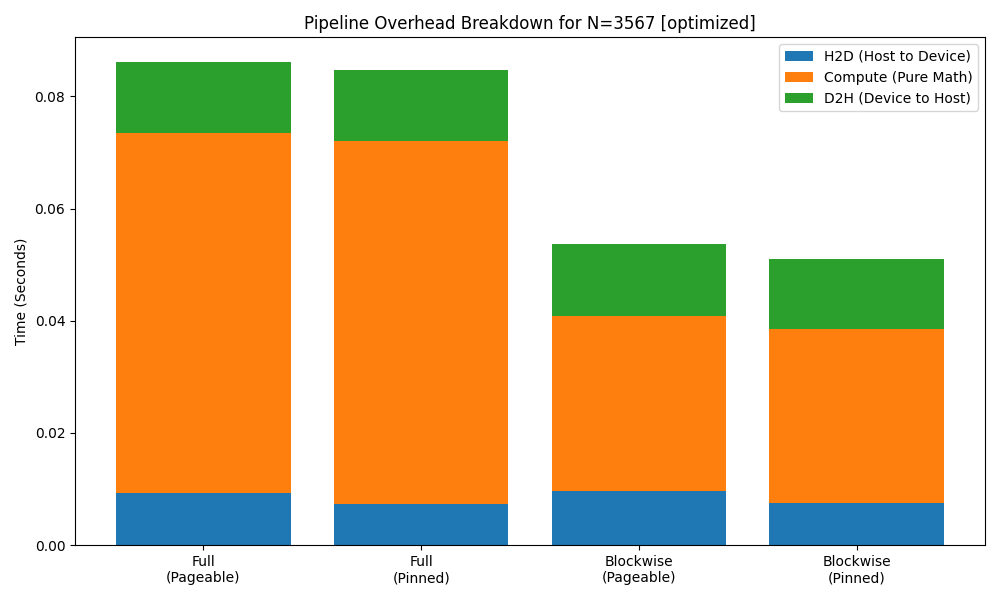
\includegraphics[width=0.45\textwidth]{figs/gpu/optimized/global_temp/global_temp_optimized_gpu_gpu_pipeline_breakdown.png}
\caption{Pipeline Overhead Breakdown: H2D vs. Compute vs. D2H for Synthetic (Left) and Real Data (Right)}
\label{fig:gpu_pipeline_breakdown}
\end{figure}

\textbf{Qualitative Observations:}
\begin{itemize}
    \item \textbf{Compute is Not the Bottleneck:} Across both datasets, the actual mathematical calculation (the middle segment of the stacked bars) accounts for a tiny fraction of the total execution time. The CUDA cores execute the $O(N^2 \cdot T)$ operations almost instantaneously.
    \item \textbf{D2H Dominance:} The Device-to-Host transfer (returning the result to the CPU) dominates the runtime. Because the output matrix space complexity $O(N^2)$ grows much faster than the input time-series data $O(N \cdot T)$, the PCIe bus bandwidth becomes the ultimate limiting factor in the system.
    \item \textbf{Amdahl's Law at Scale:} Optimizing the H2D input transfer via Pinned memory yields microsecond-level gains. However, because the standard D2H output transfer remains massively unoptimized and dominates the pipeline, the overall system speedup is severely bounded. This visually confirms the core thesis: GPU acceleration is only profitable when computational intensity heavily outweighs the physical delay of moving data across the motherboard.
\end{itemize}
\section{Conclusion and Outlook}

The development and benchmarking of the Parallel Data Processing Engine provided a rigorous evaluation of how architectural choices and algorithmic optimizations influence the processing of large-scale, high-dimensional datasets. By using the Pearson correlation matrix as a computational proxy for $O(N^2)$ complexity, several key insights were established regarding the efficiency of CPU and GPU frameworks in the context of geophysical and climate data analysis.\\

On the CPU front, the project demonstrated that hardware parallelism alone is insufficient for quadratic scaling. The implementation of symmetry-aware logic—specifically computing only the upper triangle of the matrix—provided a consistent $50\%$ reduction in total floating-point operations. This optimization proved essential for maintaining performance as the number of stations ($N$) increased. However, the gains from multi-core parallelization were frequently tempered by the ``I/O tax'' and the overhead of inter-process communication (IPC). When handling the structured NASA POWER temperature series, the ``Optimized Single-thread'' version often outperformed naive parallel versions for smaller station counts, proving that algorithmic efficiency remains the primary defense against computational bottlenecks.\\

The GPU implementation revealed a distinct performance paradigm. While initial data transfer across the PCIe bus introduced a measurable constant-time overhead, the massively parallel nature of tensor operations in PyTorch allowed the engine to achieve throughput levels orders of magnitude higher than the CPU once the ``break-even point'' was surpassed. By mapping dense matrix operations directly to CUDA cores, the engine bypassed the complex shared-memory management and process chunking required by the CPU. This makes the GPU the superior architecture for high-density geographic grids where the computational intensity of the $O(N^2 \cdot T)$ correlation task significantly outweighs the $O(N \cdot T)$ cost of data movement.\\

Ultimately, this study confirms that the optimal processing strategy is not static but is a function of the dataset’s dimensionality. For researchers analyzing moderate spatial grids, a symmetry-optimized CPU approach offers high efficiency with minimal management overhead. For global-scale climate monitoring or large-scale financial time-series analysis, the GPU’s computational density successfully amortizes the cost of data transfer. The Parallel Data Processing Engine stands as a modular and scalable tool for navigating these trade-offs, providing a robust framework for high-performance numerical analysis.

\section{Acknowledgements}
The completion of this project was made possible through the support and guidance of several individuals who provided the academic and technical framework necessary to explore the complexities of parallel computing.\\

We would like to express our sincere gratitude to our instructors, Dr. Bedartha Goswami and Dr. Kalpesh Kapoor, for their invaluable mentorship. Their insights into computational efficiency and geodynamic modeling were instrumental in shaping the objectives of this engine and encouraging us to move beyond naive implementations toward true algorithmic optimization.\\

Special thanks go to our Teaching Assistant, Amruta, for her consistent support during lab sessions, and to Karan, our Tyrone Engineer, for his essential assistance in configuring the hardware environment. Their help ensured a smooth transition from theoretical design to practical benchmarking on both CPU and CUDA-enabled architectures.\\

Finally, we would like to acknowledge the collective synergy of our group. This project was a truly collaborative endeavor; the successful transformation of a complex $O(N^2)$ problem into a functional, high-performance reality is a direct result of our shared dedication, joint problem-solving, and mutual support throughout every stage of development.

We would also like to acknowledge the AI assistance for this work. We used tools such as ChatGPT and Google Gemini for code generation, debugging, and writing assistance \cite{ai_tools_2026}.


\section{Author Contributions}

The individual contributions of the group members are outlined below based on the CRediT (Contributor Roles Taxonomy):

\begin{itemize}
    \item \textbf{Amitava Dutta}
    \begin{itemize}
        \item \textbf{Repository Architecture:} Designed the core repository structure and the unified execution framework (\texttt{run\_experiment.py}).
        \item \textbf{Software Development:} Implemented the primary CPU pipeline, including single-threaded, multi-threaded (shared-memory), and block-wise optimization modules.
        \item \textbf{System Integration:} Integrated GPU kernels into the unified CLI and modularized functional scripts for production-level workflow.
        \item \textbf{Formal Analysis:} Conducted theoretical $O(N^2)$ complexity analysis for CPU-bound operations.
        \item \textbf{Documentation:} Managed the project \texttt{README.md} and co-authored/edited the technical report.
    \end{itemize}

    \item \textbf{Sipra Subhadarsini Sahoo}
    \begin{itemize}
        \item \textbf{GPU Software Development:} Developed the CUDA-accelerated correlation logic using PyTorch tensor operations.
        \item \textbf{Algorithm Optimization:} Implemented the GPU-specific block-wise computation strategy to manage VRAM constraints for large-scale matrices.
        \item \textbf{Investigation:} Conducted performance profiling of GPU kernels across different hardware configurations.
    \end{itemize}

    \item \textbf{Bhavini Raina}
    \begin{itemize}
        \item \textbf{Validation:} Performed numerical consistency checks between CPU and GPU outputs using financial time-series datasets.
        \item \textbf{System Profiling:} Analyzed hardware-specific bottlenecks (CPU/GPU/RAM) during high-concurrency execution using financial time-series datasets.
        \item \textbf{Experimental Analysis:} Conducted formal complexity analysis and plotted empirical performance data for financial time-series datasets.
    \end{itemize}

    \item \textbf{Yashvita Subramanian}
    \begin{itemize}
        \item \textbf{Methodology \& Optimization:} Conducted bandwidth analysis and transfer overhead optimization, specifically comparing Pinned vs. Paged memory performance.
        \item \textbf{Data Curation:} Implemented and validated the engine's performance on real-world climate datasets (NASA POWER).
        \item \textbf{Writing \& Editing:} Co-authored and formatted the final technical report, focusing on the comparative analysis of hardware architectures.
    \end{itemize}
\end{itemize}

\section{Code availability}
The code for this project is available at the following GitHub repository:
\url{https://github.com/AmitavaDutta/parallel_data_processing_engine.git}.

% --------------------------------------------------------------------
% --------------------------------------------------------------------
% ---- DO NOT CHANGE THIS BLOCK OF CODE
\section{References}
\bibliography{refs}
% --------------------------------------------------------------------
% --------------------------------------------------------------------


\section{Appendix}

\subsection{Algorithms}

% ---------------------------------------------------------
% ALGORITHM 1: Baseline CPU
% ---------------------------------------------------------
\begin{minipage}{0.95\textwidth}
    \begin{algorithm}[H]
        \caption{Baseline CPU Correlation (Serial \& Multiprocessing)}
        \label{alg:baseline_cpu}
        \begin{algorithmic}[1]
        \Require Raw Dataset $X \in \mathbb{R}^{N \times T}$, Number of Workers $W$
        \Ensure Correlation Matrix $C \in \mathbb{R}^{N \times N}$
            \State $\mu \gets \frac{1}{T} \sum_{t=1}^{T} X_{:,t}$ \Comment{Compute row means}
            \State $\sigma \gets \sqrt{\frac{1}{T} \sum_{t=1}^{T} (X_{:,t} - \mu)^2}$ \Comment{Compute row std devs}
            \State $Z \gets (X - \mu) / \sigma$ \Comment{Z-score normalization}
            
            \If{$W = 1$} \Comment{Serial Mode}
                \State $C \gets \frac{Z \times Z^T}{T-1}$ \Comment{Full naive matrix multiplication}
            \Else \Comment{Multiprocessing Mode}
                \State Allocate Shared Memory for $Z$
                \State Partition $Z$ into $W$ row-chunks
                \For{each worker $w \in 1 \dots W$ \textbf{in parallel}}
                    \State $Z_{chunk} \gets \text{Extract rows for worker } w$
                    \State $C_{chunk} \gets \frac{Z_{chunk} \times Z^T}{T-1}$ \Comment{Redundant lower-triangle calc}
                    \State Return $C_{chunk}$
                \EndFor
                \State $C \gets \text{Vertical Stack of all } C_{chunk}$
            \EndIf
        \end{algorithmic}
    \end{algorithm}
\end{minipage}

\vspace{0.5cm}

% ---------------------------------------------------------
% ALGORITHM 2: Optimized CPU (Symmetry Aware)
% ---------------------------------------------------------
\begin{minipage}{0.95\textwidth}
    \begin{algorithm}[H]
        \caption{Optimized Multiprocessing CPU Engine (Symmetry Aware)}
        \label{alg:optimized_cpu}
        \begin{algorithmic}[1]
        \Require Normalized Dataset $Z \in \mathbb{R}^{N \times T}$, Workers $W$
        \Ensure Correlation Matrix $C \in \mathbb{R}^{N \times N}$
            \State Allocate Shared Memory for $Z$
            \State Initialize empty $C \in \mathbb{R}^{N \times N}$
            \State Partition index range $0 \dots N$ into $W$ chunks
            
            \For{each chunk starting at $idx_{start}$ to $idx_{end}$ \textbf{in parallel}}
                \State Initialize local block $C_{local}$
                \For{$i$ from $idx_{start}$ to $idx_{end}-1$}
                    \For{$j$ from $i$ to $N-1$} \Comment{Exploit Symmetry: Upper Triangle Only}
                        \State $C_{local}[i, j] \gets \frac{Z_i \cdot Z_j}{T-1}$ 
                    \EndFor
                    \State $C_{local}[i, i] \gets 1.0$ \Comment{Exploit Identity Diagonal}
                \EndFor
                \State Return $C_{local}$
            \EndFor
            
            \State Assemble $C_{local}$ blocks into upper portion of $C$
            \For{all $j < i$} \Comment{Mirror lower triangle}
                \State $C[j, i] \gets C[i, j]$ 
            \EndFor
        \end{algorithmic}
    \end{algorithm}
\end{minipage}

\vspace{0.5cm}

% ---------------------------------------------------------
% ALGORITHM 3: Block-wise CPU (Cache Optimized)
% ---------------------------------------------------------
\begin{minipage}{0.95\textwidth}
    \begin{algorithm}[H]
        \caption{Cache-Optimized Block-wise Correlation}
        \label{alg:block_cpu}
        \begin{algorithmic}[1]
        \Require Normalized Dataset $Z \in \mathbb{R}^{N \times T}$, Block Size $B$
        \Ensure Correlation Matrix $C \in \mathbb{R}^{N \times N}$
            \State Initialize empty $C \in \mathbb{R}^{N \times N}$
            
            \For{$i = 0, B, 2B \dots N-1$}
                \State $Z_i \gets Z[i : i+B]$ \Comment{Load row block into cache}
                
                \For{$j = i, i+B \dots N-1$} \Comment{Upper Triangle of Blocks}
                    \State $Z_j \gets Z[j : j+B]$
                    \State $C_{block} \gets \frac{Z_i \times Z_j^T}{T-1}$ \Comment{Saturated BLAS block operation}
                    
                    \State $C[i:i+B, \ j:j+B] \gets C_{block}$
                    
                    \If{$i \neq j$} \Comment{Mirror off-diagonal blocks}
                        \State $C[j:j+B, \ i:i+B] \gets C_{block}^T$
                    \EndIf
                \EndFor
            \EndFor
        \end{algorithmic}
    \end{algorithm}
\end{minipage}

\vspace{0.5cm}

% ---------------------------------------------------------
% ALGORITHM 4: GPU Accelerated
% ---------------------------------------------------------
\begin{minipage}{0.95\textwidth}
    \begin{algorithm}[H]
        \caption{Full GPU Tensor Acceleration Engine}
        \label{alg:gpu_full}
        \begin{algorithmic}[1]
        \Require Host Dataset $X_{cpu} \in \mathbb{R}^{N \times T}$, Target Device $GPU$
        \Ensure Host Correlation Matrix $C_{cpu} \in \mathbb{R}^{N \times N}$
            \State $X_{gpu} \gets \text{Transfer } X_{cpu} \text{ to } GPU$ VRAM
            \State $\mu_{gpu} \gets X_{gpu}\text{.mean(dim=1)}$ \Comment{Parallel reduction on device}
            \State $\sigma_{gpu} \gets X_{gpu}\text{.std(dim=1)}$ 
            \State $\sigma_{gpu} \gets \text{clamp}(\sigma_{gpu}, \text{min}=10^{-8})$ \Comment{Prevent division by zero}
            
            \State $Z_{gpu} \gets (X_{gpu} - \mu_{gpu}) / \sigma_{gpu}$
            
            \State $C_{gpu} \gets \frac{Z_{gpu} \times Z_{gpu}^T}{T}$ \Comment{Massively parallel tensor multiplication}
            \State $C_{gpu} \gets \text{clamp}(C_{gpu}, -1.0, 1.0)$ \Comment{Floating point error correction}
            
            \State $C_{cpu} \gets \text{Transfer } C_{gpu} \text{ back to Host RAM}$
            \State Clear GPU Cache
        \end{algorithmic}
    \end{algorithm}
\end{minipage}


\subsection{Code Snippets}

While the complete source code and CLI orchestration scripts are available in the accompanying repository, this section highlights two critical computational kernels that define the performance characteristics of our engine. 

\subsubsection*{1. Symmetry-Aware CPU Implementation}
This snippet from \verb|parallel_cpu.py| demonstrates the optimized multiprocessing logic. Rather than computing the full $N \times N$ matrix redundantly, the inner loop strictly restricts computation to the upper triangle (\verb|range(i, N)|) and manually assigns the identity diagonal, effectively cutting the computational debt in half.

\begin{minted}[bgcolor=white, fontsize=\small, linenos, frame=none]{python}
def _compute_chunk_optimized(args):
    shm_name, shape, dtype, start_idx, end_idx, T = args
    
    # ... Shared memory buffer initialization omitted ...
    
    N = shape[0]
    result = np.zeros((end_idx - start_idx, N), dtype=dtype)

    for local_i, i in enumerate(range(start_idx, end_idx)):
        Zi = Z[i]

        # OPTIMIZATION: Compute upper triangle only
        for j in range(i, N):  
            result[local_i, j] = np.dot(Zi, Z[j]) / (T - 1)

        # OPTIMIZATION: Exploit identity diagonal
        result[local_i, i] = 1.0

    return (start_idx, result)
\end{minted}

\vspace{0.5cm}

\subsubsection*{2. Massively Parallel GPU Tensor Logic}
This snippet from \verb|gpu_correlation.py| showcases the elegant simplicity of hardware acceleration using PyTorch. The complex shared-memory management and process chunking required by the CPU are entirely bypassed. The normalization and dot-product operations are mapped directly to CUDA cores as dense tensor operations.

\begin{minted}[bgcolor=white, fontsize=\small, linenos, frame=none]{python}
def gpu_correlation_full(data: np.ndarray, device: torch.device):
    # Load data onto GPU VRAM
    X = torch.tensor(data, device=device)
    
    # Massively parallel Z-score normalization
    mean = X.mean(dim=1, keepdim=True)
    std = torch.std(X, dim=1, keepdim=True, unbiased=False)
    std = torch.clamp(std, min=1e-8) # Prevent division by zero
    Z = (X - mean) / std

    T = data.shape[1]
    
    # Core Operation: Dense Matrix Multiplication via cuBLAS
    C = torch.mm(Z, Z.T) / T
    
    # Floating point error correction
    C = torch.clamp(C, -1.0, 1.0) 

    return C
\end{minted}


% --------------------------------------------------------------------
% --------------------------------------------------------------------
% ---- DO NOT CHANGE THIS BLOCK OF CODE
\end{document}
% --------------------------------------------------------------------
% --------------------------------------------------------------------